%% Pasado
%%

\definecolor{lightviolet}{HTML}{F4AFF4}
\definecolor{lightorange}{HTML}{FFA17F}
\definecolor{lightgreen}{HTML}{98FB98}
\definecolor{lightred}{HTML}{FF5C5C}
\definecolor{lightblue}{HTML}{89AFCF}
\definecolor{lightbrown}{HTML}{B58868}

%%-----------------------------------------
%%-----------------------------------------
\section{Pasado}

\begin{flushright}
{\em
  ¿Quiénes somos? \\
  ¿De dónde venimos? \\
  ¿Adónde vamos? \\
}
~ \\
Siniestro Total \\
\end{flushright}


%%-----------------------------------------
\begin{frame}[fragile]
  \frametitle{La suerte de estar en el sitio adecuado}

  \begin{center}
  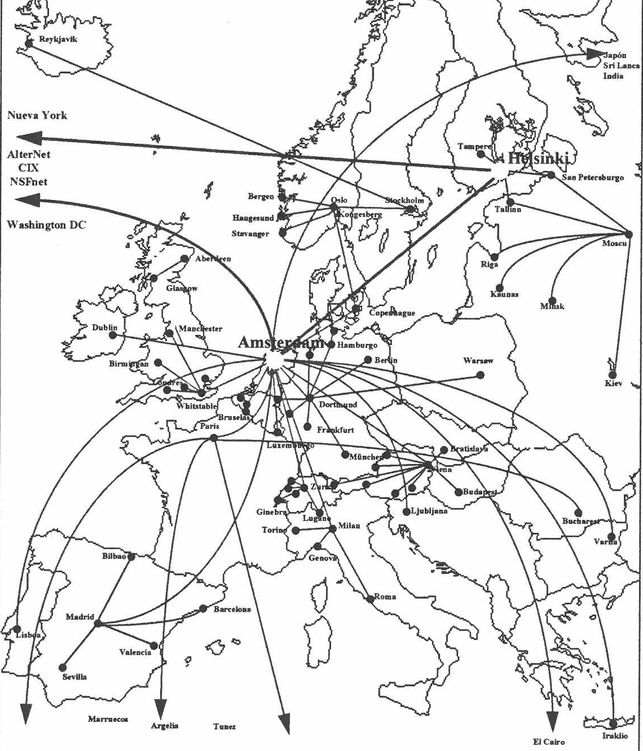
\includegraphics[height=6cm]{figs/eunet}
  \end{center}  
  
\end{frame}

%%-----------------------------------------
\begin{frame}[fragile]
  \frametitle{La suerte de estar en el momento adecuado}

  \begin{center}
  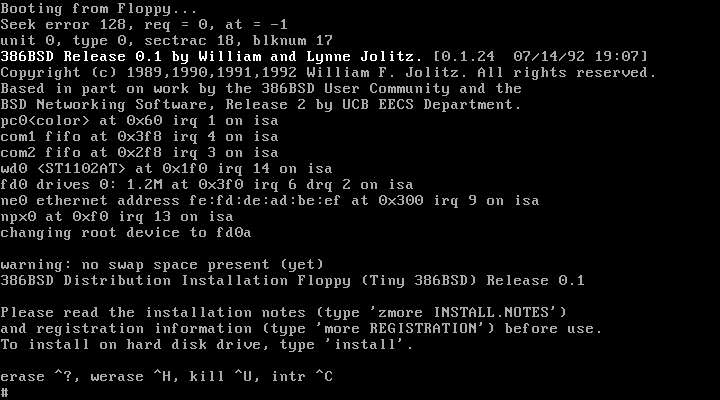
\includegraphics[height=6cm]{figs/386BSD-installer}
  \end{center}  
  
\end{frame}

%%-----------------------------------------
\begin{frame}[fragile]
  \frametitle{La suerte de tener buenos maestros}

  \begin{center}
  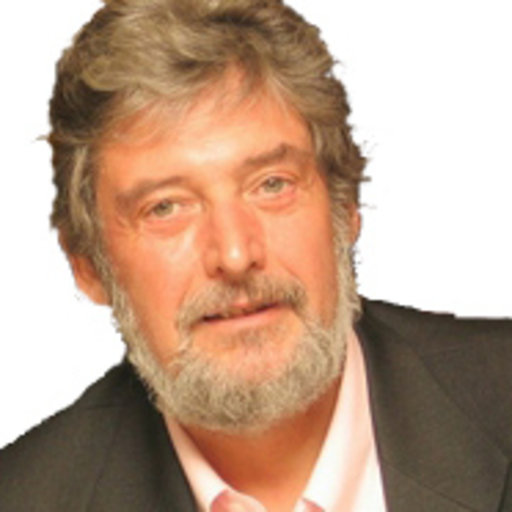
\includegraphics[height=3.5cm]{figs/foto-aalvarez}
  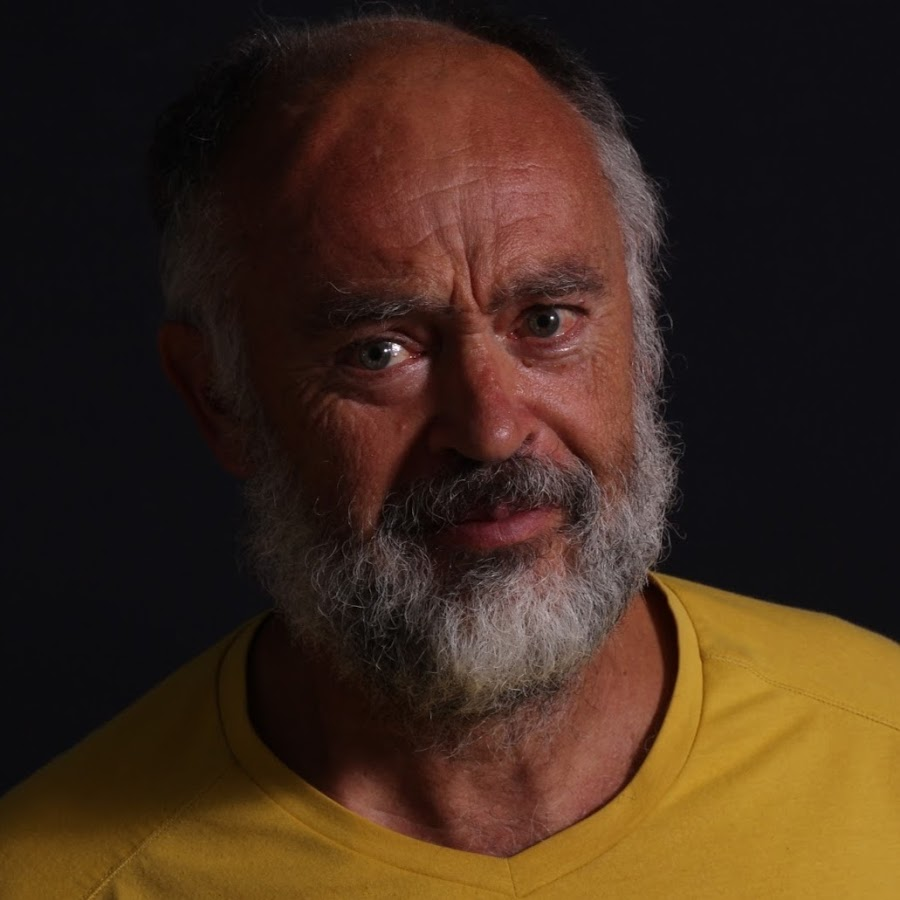
\includegraphics[height=3.5cm]{figs/foto-jseoane}
  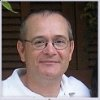
\includegraphics[height=3.5cm]{figs/foto-sarevalo}
  \end{center}  
  
\end{frame}

%%-----------------------------------------
\begin{frame}[fragile]
  \frametitle{La suerte de que te hayan preparado el camino}

  \begin{center}
  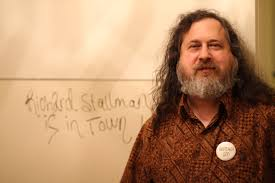
\includegraphics[height=6cm]{figs/foto-rms}
  \end{center}  
  
\end{frame}

%%-----------------------------------------
\begin{frame}[fragile]
  \frametitle{Mi vida (académica)}

  % Definition of the chronology element
%  \startchronology[align=left, startyear=1986,stopyear=2017, height=0pt, startdate=false, stopdate=false, dateselevation=0pt, arrow=false, box=true]
  %
  %  \chronograduation[event][dateselevation=0pt]{1}
  \startchronology[startyear=1984,stopyear=2017,dates=false,color=white]
  % Periods and events

  \chronoperiode[textstyle=\raggedleft\colorbox{gray!30}, color=gray, startdate=false, bottomdepth=0pt, topheight=8pt, textdepth=-25pt,dateselevation=16pt, stopdate=false]{1986}{1992}{Ing. Telecom (UPM)}

  \chronoevent[colorbox=gray!30,conversionmonth=false, datesseparation=/, markdepth=3cm]{12/1991}{Ing. Telecomunicación (UPM)}

  \chronoperiode[textstyle=\raggedleft\colorbox{gray!30}, color=gray, startdate=false, bottomdepth=0pt, topheight=8pt, textdepth=-45pt,dateselevation=16pt, stopdate=false]{1993}{1999}{Doctorado (UPM)}

  \chronoevent[colorbox=gray!30,conversionmonth=false,datesseparation=/, markdepth=1.5cm]{12/1998}{Doctor Ing. Telecomunicación}

  \chronoperiode[textstyle=\colorbox{lightviolet}, color=lightviolet, startdate=false, bottomdepth=10pt, topheight=18pt, textdepth=-55pt, dateselevation=12pt,stopdate=false]{1992}{2000}{UC3M}

  \chronoperiode[textstyle=\colorbox{lightviolet}, color=lightviolet, startdate=false, bottomdepth=10pt, topheight=18pt, textdepth=-55pt, dateselevation=12pt,stopdate=false]{2000}{2017}{URJC}

  \chronoevent[colorbox=gray!30,conversionmonth=false,datesseparation=/, markdepth=.1cm]{05/2001}{Plaza TU}

  \chronoevent[colorbox=gray!30,conversionmonth=false,datesseparation=/, markdepth=.1cm]{05/2015}{Habilitación CU}

  \stopchronology

\end{frame}


%%-----------------------------------------
\begin{frame}[fragile]
  \frametitle{Una vida docente}

  {\small
  ~~~~~~~UCAR~~~~~~~~~~~~~~~~~~~~~~~~~~~~~~~URJC
  }
  
  \vspace{.2cm}
  
  {\footnotesize
  \startchronology[startyear=1992,stopyear=2018,dates=true, color=white, width=.9\textwidth]

  % UC3M Informatica
  \chronoperiode[color=lightred, startdate=false, stopdate=false, bottomdepth=0pt, topheight=8pt]{1992}{1999}{}

  \chronoevent[barre=false, colorbox=lightred, markdepth=1.2cm, date=false, textwidth=2.4cm]{1/1995}{Informática}

  % UC3M Industriales
  \chronoperiode[color=lightred, startdate=false, stopdate=false, bottomdepth=10pt, topheight=18pt]{1997}{1999}{}

  \chronoevent[barre=false, colorbox=lightred, markdepth=.7cm, date=false, textwidth=1.9cm]{1/1998}{Industriales}

  % UC3M Doctorado
  \chronoperiode[color=lightgreen, startdate=false, stopdate=false, bottomdepth=20pt, topheight=28pt]{1997}{1999}{}

  \chronoevent[barre=false, colorbox=lightgreen, markdepth=.2cm, date=false, textwidth=1.9cm]{1/1998}{Doctorado}

  % URJC Grado Ciencias Salud
  \chronoperiode[color=lightred, startdate=false, stopdate=false, bottomdepth=60pt, topheight=68pt]{1999}{2005}{}

  \chronoevent[barre=false, colorbox=lightred, markdepth=1.6cm, date=false, textwidth=2cm]{7/2001}{C. Salud}

  % URJC Grado Informática
  \chronoperiode[color=lightred, startdate=false, stopdate=false, bottomdepth=70pt, topheight=78pt]{1999}{2011}{}

  \chronoevent[barre=false, colorbox=lightred, markdepth=1.2cm, date=false, textwidth=2.5cm]{1/2005}{Informática}

  % URJC Grado Teleco
  \chronoperiode[color=lightred, startdate=false, stopdate=false, bottomdepth=80pt, topheight=88pt]{2003}{2018}{}

  \chronoevent[barre=false, colorbox=lightred, markdepth=1.6cm, date=false, textwidth=2cm]{1/2010}{Teleco}

  % URJC Doctorado Informatica
  \chronoperiode[color=lightgreen, startdate=false, stopdate=false, bottomdepth=30pt, topheight=38pt]{2001}{2006}{}

  \chronoevent[barre=false, colorbox=lightgreen, markdepth=.2cm, date=false, textwidth=1.9cm]{7/2003}{Doctorado}

  % URJC Máster RSCM URJC
  \chronoperiode[color=lightviolet, startdate=false, stopdate=false, bottomdepth=40pt, topheight=48pt]{2006}{2011}{}

  \chronoevent[barre=false, colorbox=lightviolet, markdepth=.7cm, date=false, textwidth=2.5cm]{7/2008}{Máster RSCM}

  % URJC Máster Software Libre URJC
  \chronoperiode[color=lightviolet, startdate=false, stopdate=false, bottomdepth=50pt, topheight=58pt]{2006}{2014}{}

  \chronoevent[barre=false, colorbox=lightviolet, markdepth=.2cm, date=false, textwidth=1.9cm]{1/2009}{Máster SL}



  \stopchronology
  }
\end{frame}



%%-----------------------------------------
\begin{frame}[fragile]
  \frametitle{UC3M (1992-1999)}

  \begin{center}
  
\includegraphics[height=8cm]{figs/inf-uc3m}
  \end{center}  
  
\end{frame}

%%-----------------------------------------
\begin{frame}[fragile]
  \frametitle{Laboratorios con software libre (1993-2005)}

  \begin{center}
  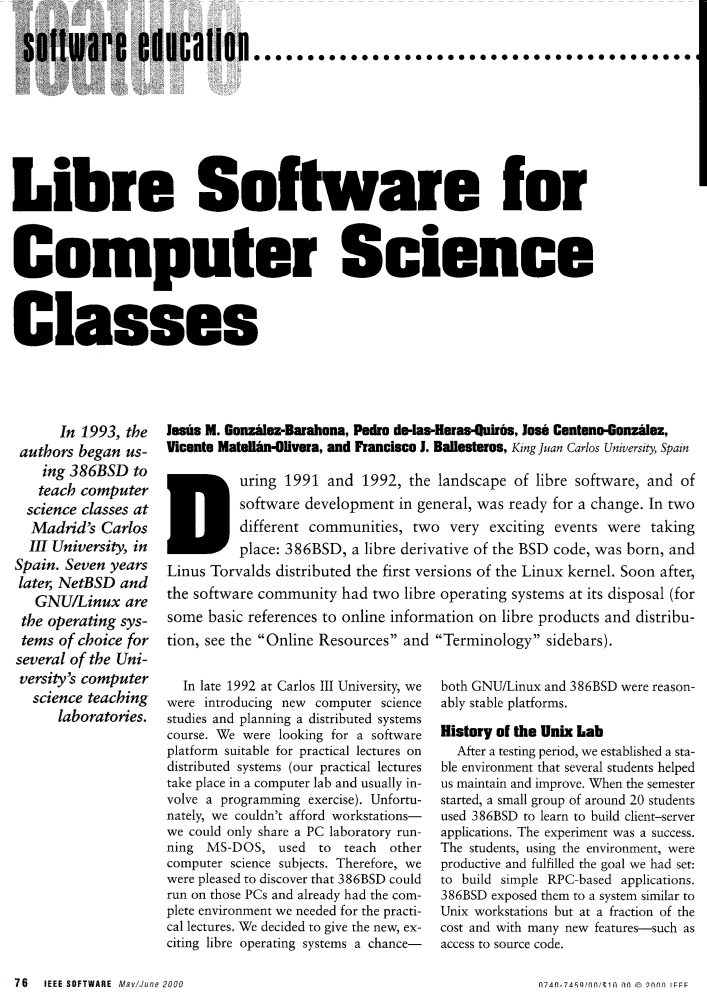
\includegraphics[height=8cm]{figs/libre-classes}
  \end{center}  
  
\end{frame}

%%-----------------------------------------
\begin{frame}[fragile]
  \frametitle{GSyC (1995-)}

  \begin{center}
  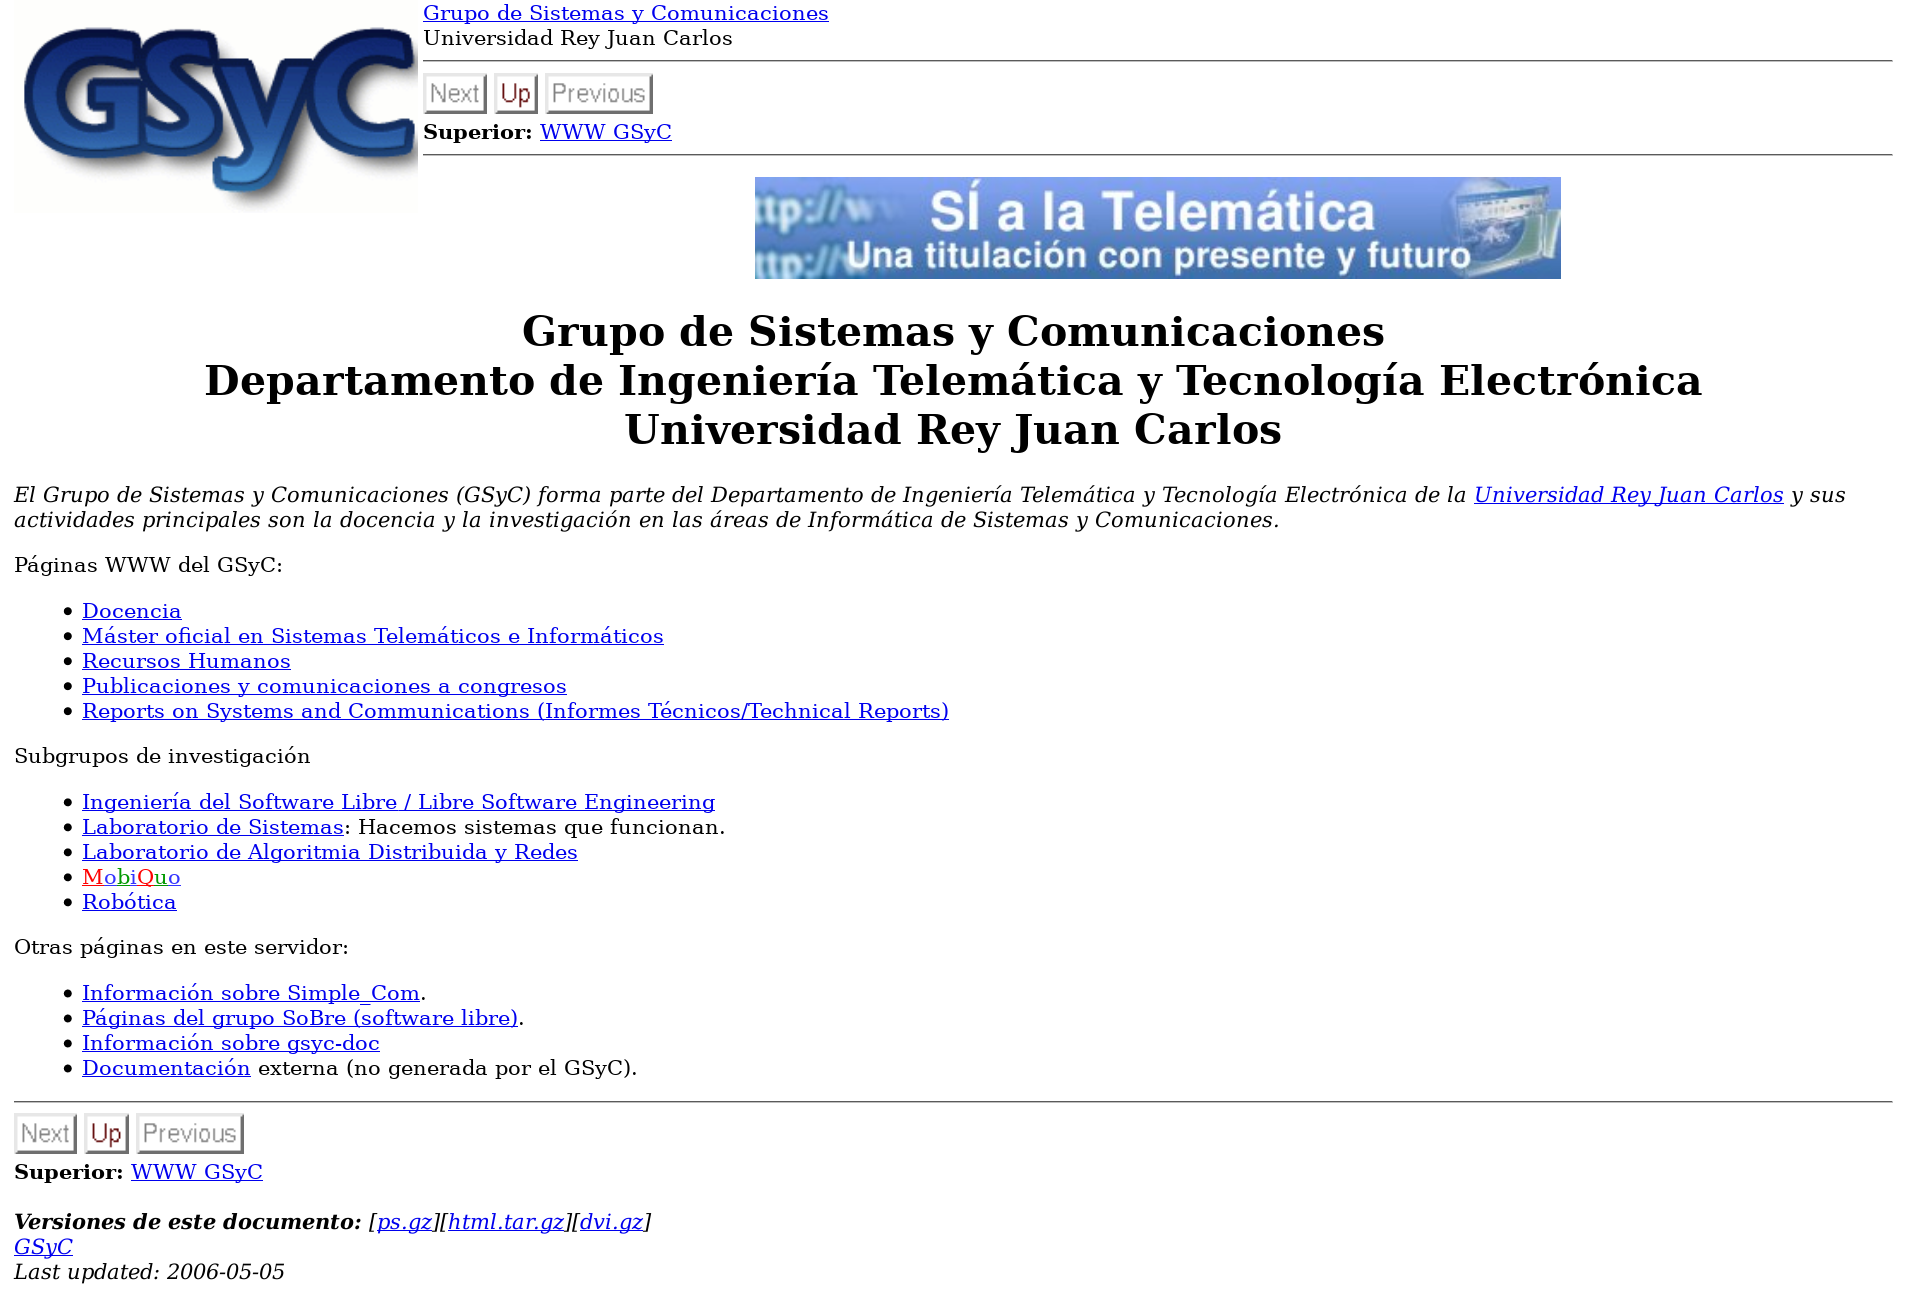
\includegraphics[height=8cm]{figs/gsyc}
  \end{center}  
  
\end{frame}

%%-----------------------------------------
\begin{frame}[fragile]
  \frametitle{Tesis y Lower\_Layer (1995-2002)}

  \begin{center}
  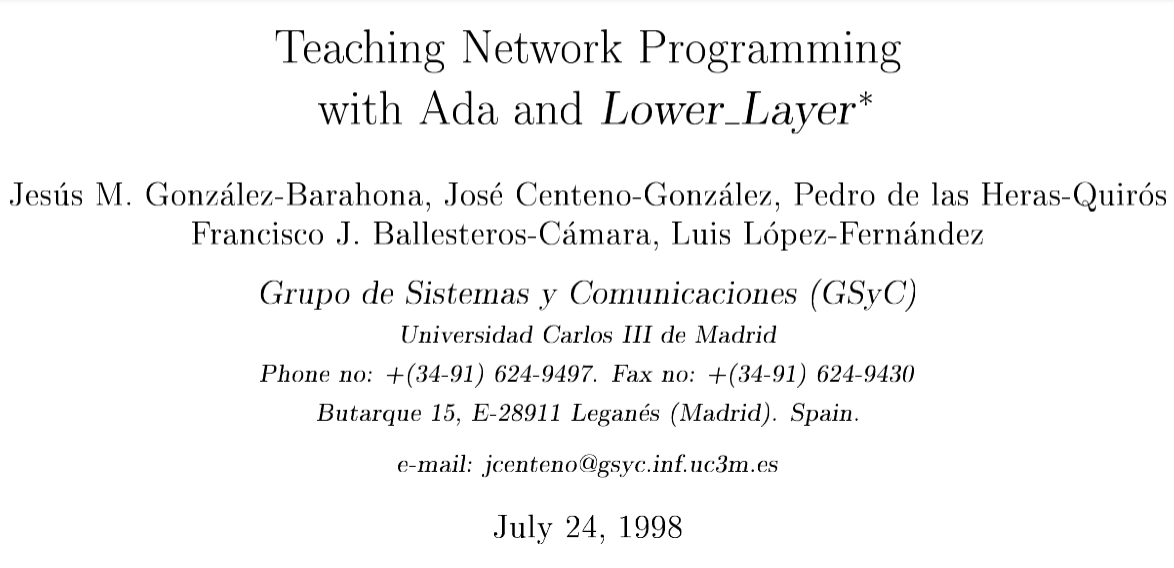
\includegraphics[width=12cm]{figs/lower-layer}
  \end{center}  
  
\end{frame}

%%-----------------------------------------
\begin{frame}[fragile]
  \frametitle{ESCET (URJC) (1999-2011)}

  \begin{center}
  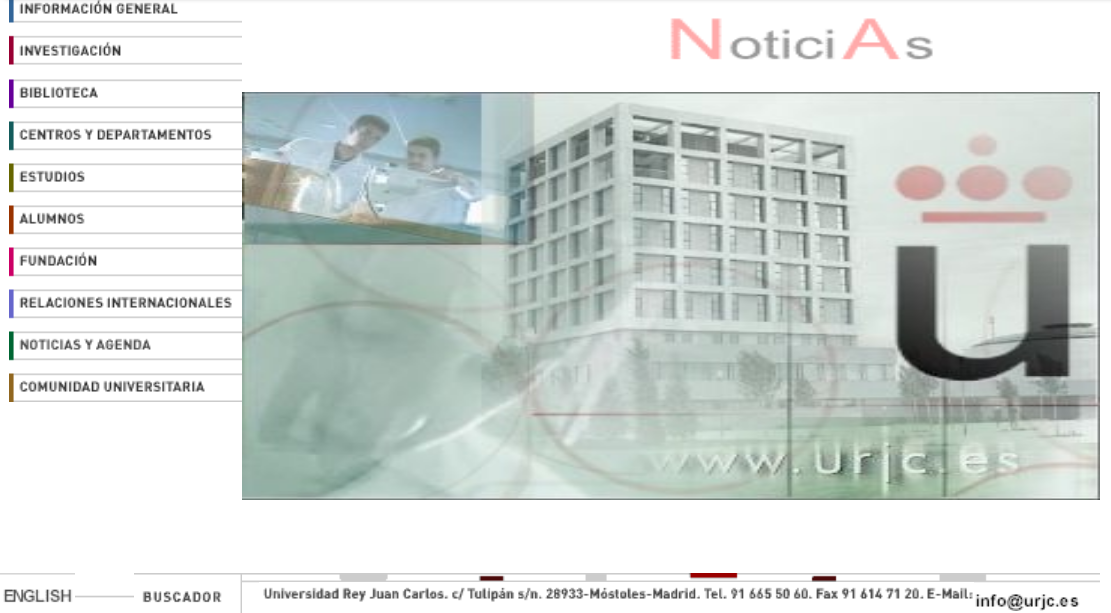
\includegraphics[width=11cm]{figs/web-urjc-2001}
  \end{center}  
  
\end{frame}

%%-----------------------------------------
\begin{frame}[fragile]
  \frametitle{Countando patatas (2000-2001)}

  \begin{center}
  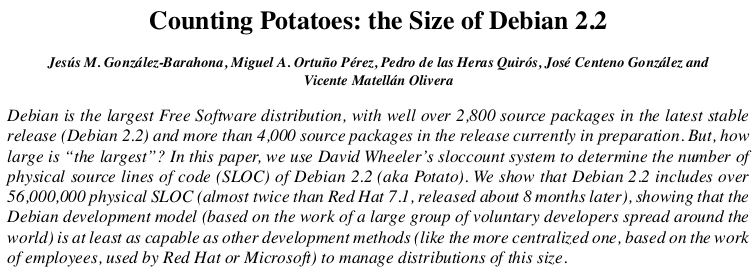
\includegraphics[width=12cm]{figs/counting-potatos}

  
\includegraphics[width=6cm]{figs/upgrade}
  \end{center}  
  
\end{frame}

%%-----------------------------------------
\begin{frame}[fragile]
  \frametitle{Uso de datos de CVS (2001-2003)}

  \begin{center}
  
\includegraphics[width=12cm]{figs/evolution-data}
  \end{center}  
  
\end{frame}

%%-----------------------------------------
\begin{frame}[fragile]
  \frametitle{CVSAnalY (2002-2015)}

  \begin{center}
  
\includegraphics[width=12cm]{figs/cvsanaly}
  \end{center}  
  
\end{frame}

%%-----------------------------------------
\begin{frame}[fragile]
  \frametitle{ETSIT (URJC) (2003-)}

  \begin{center}
  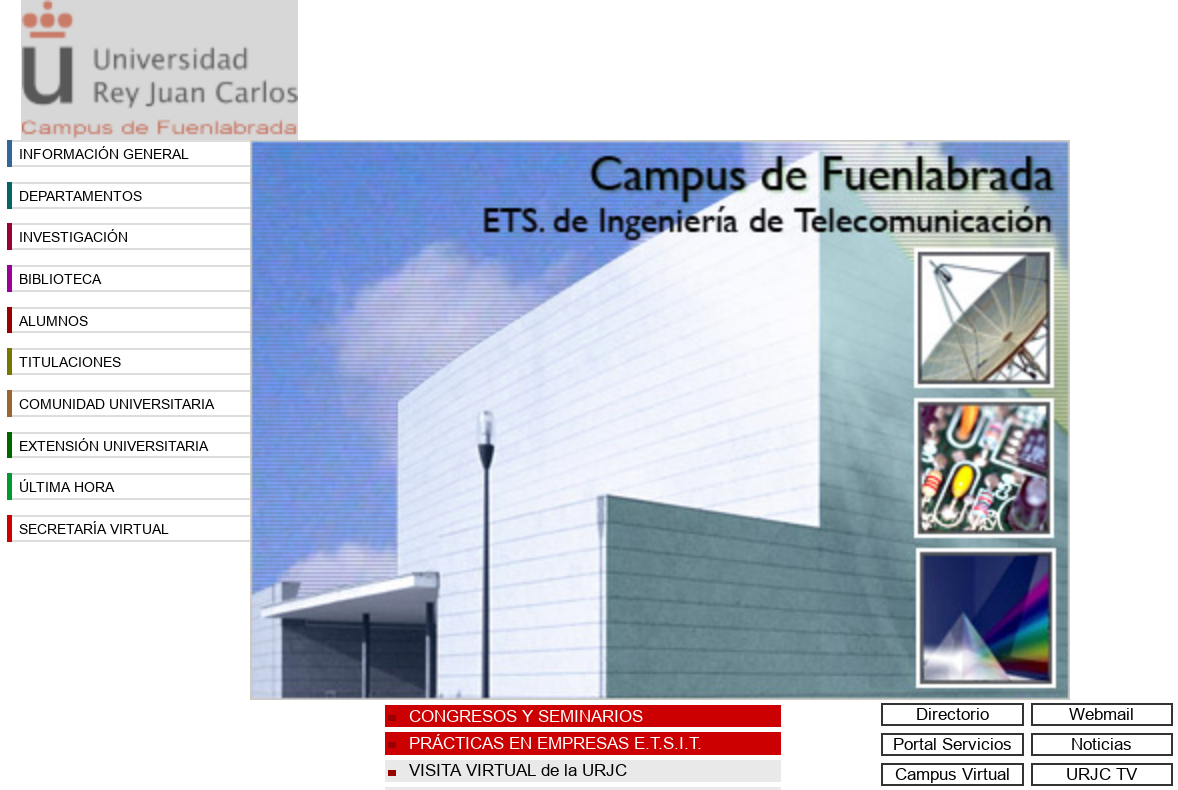
\includegraphics[width=12cm]{figs/etsit-urjc}
  \end{center}  
  
\end{frame}

%%-----------------------------------------
\begin{frame}[fragile]
  \frametitle{Software libre en Europa (2005)}

  \begin{center}
  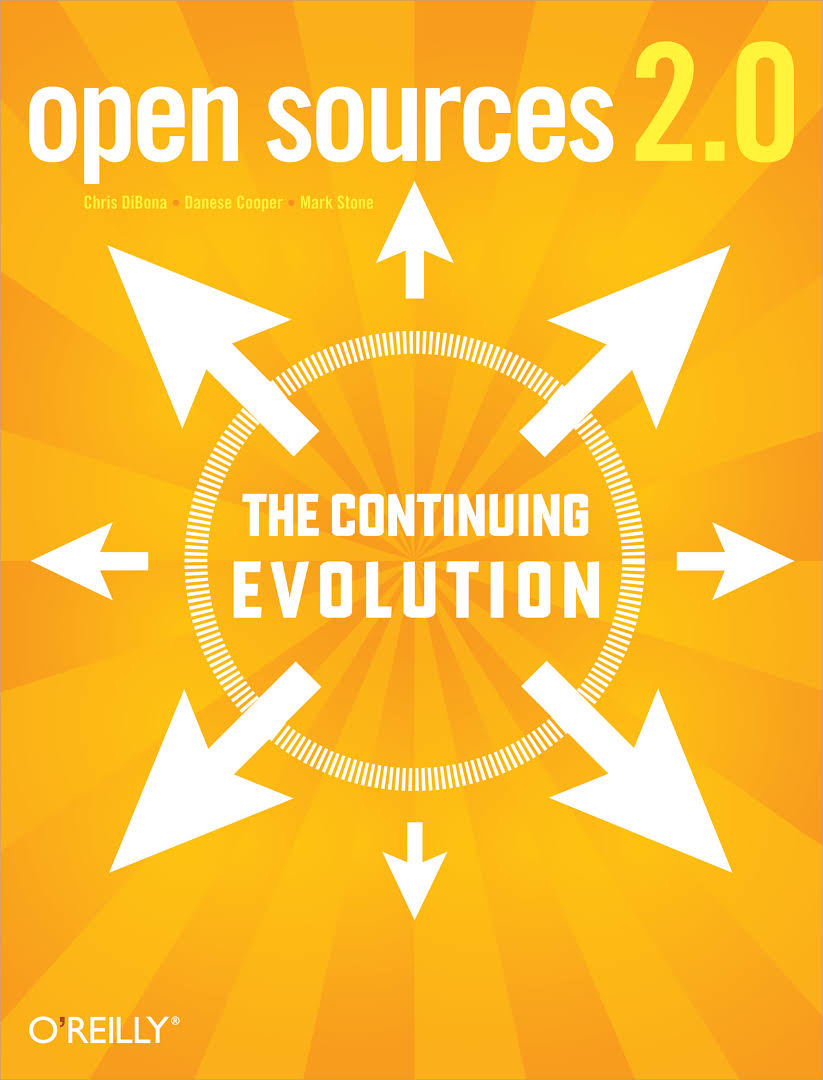
\includegraphics[height=8cm]{figs/opensources}
  \end{center}  
  
\end{frame}

%%-----------------------------------------
\begin{frame}[fragile]
  \frametitle{Mejor artículo (2000-2006)}

  \begin{center}
  
\includegraphics[height=8cm]{figs/msr-best-paper}
  \end{center}  
  
\end{frame}

%%-----------------------------------------
\begin{frame}[fragile]
  \frametitle{Macro-evolución (2005-2008)}

  \begin{center}
  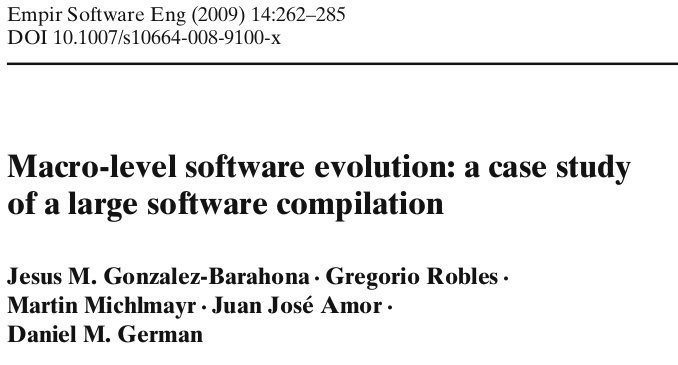
\includegraphics[width=12cm]{figs/macro-evolution}
  \end{center}  
  
\end{frame}

%%-----------------------------------------
\begin{frame}[fragile]
  \frametitle{Docencia sobre software libre (2002-2008)}

  \begin{center}
  
\includegraphics[width=12cm]{figs/intro-sobre}
  \end{center}  
  
\end{frame}

%%-----------------------------------------
\begin{frame}[fragile]
  \frametitle{FLOSSMetrics (2006-2009)}

  \begin{center}
  
\includegraphics[width=12cm]{figs/flossmetrics}
  \end{center}  
  
\end{frame}

%%-----------------------------------------
\begin{frame}[fragile]
  \frametitle{Estudios sobre Wikipedia (2007-2009)}

  \begin{center}
  
\includegraphics[width=12cm]{figs/wikipedia}
  \end{center}  
  
\end{frame}

%%-----------------------------------------
\begin{frame}[fragile]
  \frametitle{Reproducibilidad (2008-2012)}

  \begin{center}
  
\includegraphics[width=12cm]{figs/reproducibility}
  \end{center}  
  
\end{frame}

%%-----------------------------------------
\begin{frame}[fragile]
  \frametitle{Evolución basada en datos (2008-2013)}

  \begin{center}
  
\includegraphics[width=12cm]{figs/evolution-data}
  \end{center}  
  
\end{frame}

%%-----------------------------------------
\begin{frame}[fragile]
  \frametitle{Empresas y comunidades (2010-2013)}

  \begin{center}
  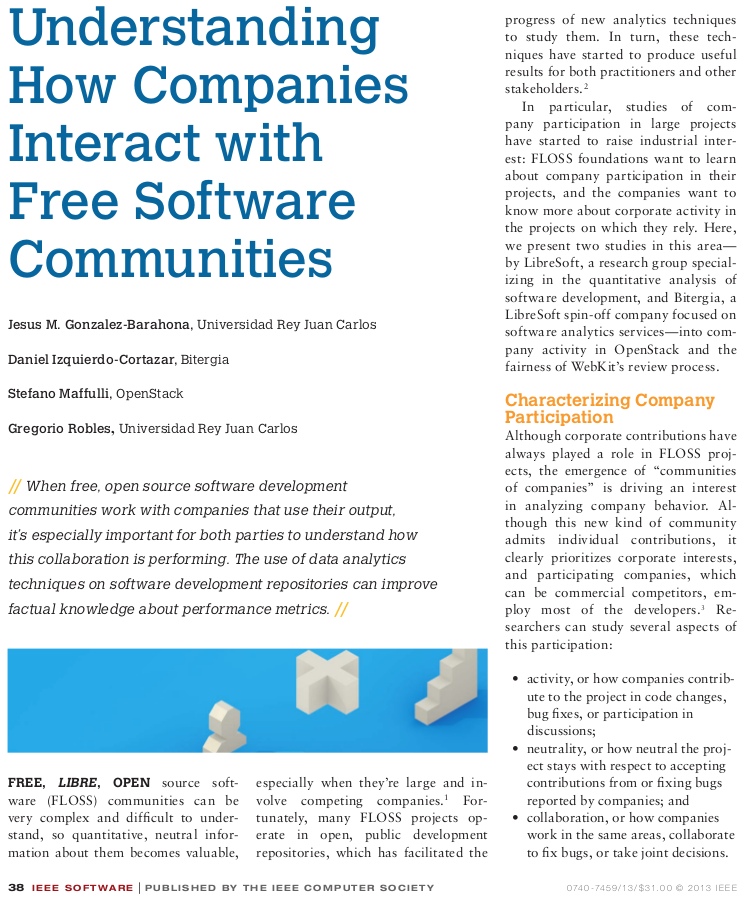
\includegraphics[width=12cm]{figs/software-companies}
  \end{center}  
  
\end{frame}

%%-----------------------------------------
\begin{frame}[fragile]
  \frametitle{MetricsGrimoire (2002-2015)}

  \begin{center}
  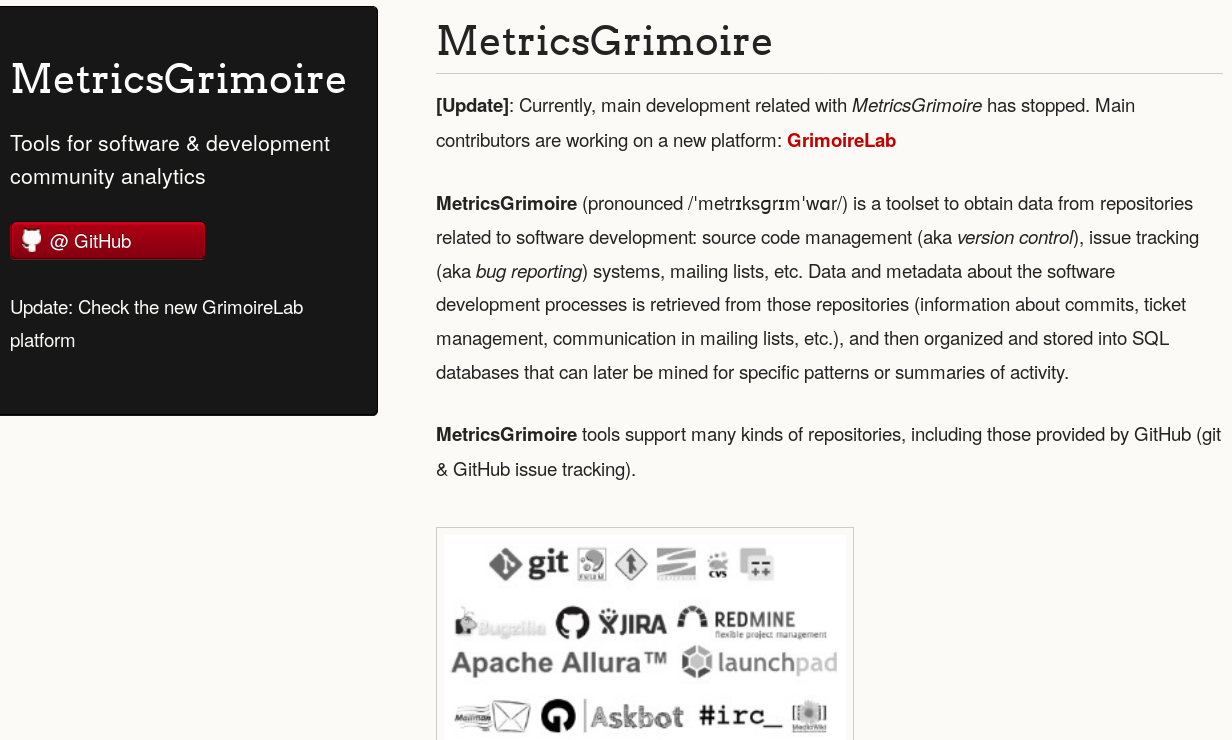
\includegraphics[width=12cm]{figs/metricsgrimoire}
  \end{center}  
  
\end{frame}

%%-----------------------------------------
\begin{frame}[fragile]
  \frametitle{Bitergia (2012-)}

  \begin{center}
  
\includegraphics[width=12cm]{figs/bitergia}
  \end{center}  
  
\end{frame}

%%-----------------------------------------
\begin{frame}[fragile]
  \frametitle{GrimoireLab (2014-)}

  \begin{center}
  
\includegraphics[width=12cm]{figs/grimoirelab}
  \end{center}  
  
\end{frame}
